\documentclass[12pt, twoside]{article}
\usepackage[letterpaper, margin=1in, headsep=0.5in]{geometry}
\usepackage[english]{babel}
\usepackage[utf8]{inputenc}
\usepackage{amsmath}
\usepackage{amsfonts}
\usepackage{amssymb}
\usepackage{tikz}
%\usetikzlibrary{quotes, angles}

\usepackage{graphicx}
\usepackage{enumitem}
\usepackage{multicol}

\usepackage{fancyhdr}
\pagestyle{fancy}
\fancyhf{}
\renewcommand{\headrulewidth}{0pt} % disable the underline of the header

\fancyhead[RE]{\thepage}
\fancyhead[RO]{\thepage \\ Name: \hspace{3cm}}
\fancyhead[L]{BECA / Dr. Huson / 10th Grade Geometry\\* 2 January 2019}

\begin{document}
\subsubsection*{Classwork: Happy New Year! \\ \qquad Due at the end of class}
 \begin{enumerate}

  \begin{multicols}{2}
    [\item A rotation of $90^\circ$ around the vertex $B$ of triangle $ABC$ carries it onto triangle $DEF$.] \vspace{0.5cm}
      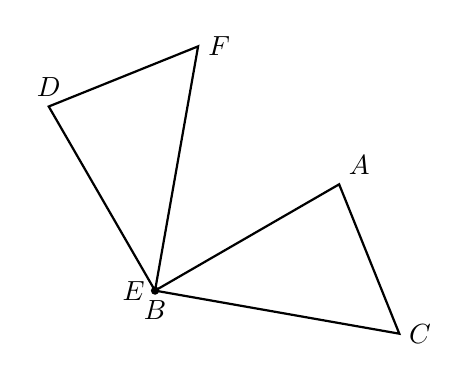
\begin{tikzpicture}[scale=0.9]
        \coordinate [label=above right:$A$](A) at (30:3);
        \coordinate [label=below:$B$](B) at (0, 0);
        \coordinate [label=right:$C$](C) at (-10:3.5);
        \draw [thick] (A)--(B)--(C)--cycle;
            \draw [fill] (0,0) circle [radius=0.05];
        \draw [thick, rotate=90] (30:3) node[above]{$D$}--
        (0,0) node[left]{$E$}--
        (-10:3.5) node[right]{$F$}--cycle;
      \end{tikzpicture}\\
      Fill in the blank with the corresponding object.
      \begin{enumerate}
        \item $A \rightarrow$ \rule{2cm}{0.15mm} \vspace{0.3cm}
        \item $\angle ABC \cong$ \rule{2cm}{0.15mm}  \vspace{0.3cm}
        \item \rule{2cm}{0.15mm} $\cong \overline {EF}$ \vspace{0.3cm}
        \item Justify that the areas of $\triangle ABC$ and $\triangle DEF$ are equal. Use the words, ``rotation," ``rigid motion," and ``preserves distance." \vspace{2cm}
      \end{enumerate}
    \end{multicols} \vspace{4cm}

    \item State the transformation that carries the trapezoid $BECA$, onto $B'E'C'A'$, as shown below. \\
      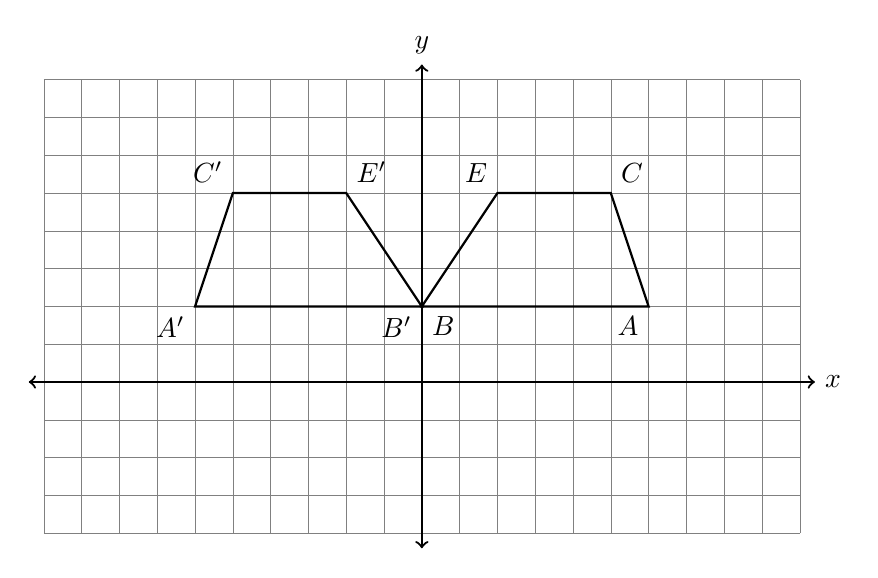
\begin{tikzpicture}[scale=.48]
        \draw [help lines] (-10,-4) grid (10,8);
        \draw [thick, <->] (-10.4,0) -- (10.4,0) node [right] {$x$};
        \draw [thick, <->] (0,-4.4)--(0,8.4) node [above] {$y$};

        \draw [thick]
        (0,2) node[below right] {$B$}--
        (2,5) node[above left] {$E$}--
        (5,5) node[above right] {$C$}--
        (6,2) node[below left] {$A$}--cycle;

        \draw [thick]
        (0,2) node[below left] {$B'$}--
        (-2,5) node[above right] {$E'$}--
        (-5,5) node[above left] {$C'$}--
        (-6,2) node[below left] {$A'$}--cycle;
      \end{tikzpicture}

        Note: For translations, you must state the $x$ and $y$ quantities; for reflections, the line of reflection; for rotations, the center of rotation and quantity in degrees.
\newpage

   \item The vertices of $\triangle JKL$ have the coordinates $J(-4,-2)$, $K(-5,1)$, and $L(-2,3)$, as shown below. \\[0.5cm]
   Apply a translation of $(x,y) \rightarrow (x+6, y-7)$ to $\triangle JKL$ and then reflect the image across the $y$-axis. Draw both images $\triangle J'K'L'$ and $\triangle J''K''L''$ on the set of axes below, labeling the vertices.\\
     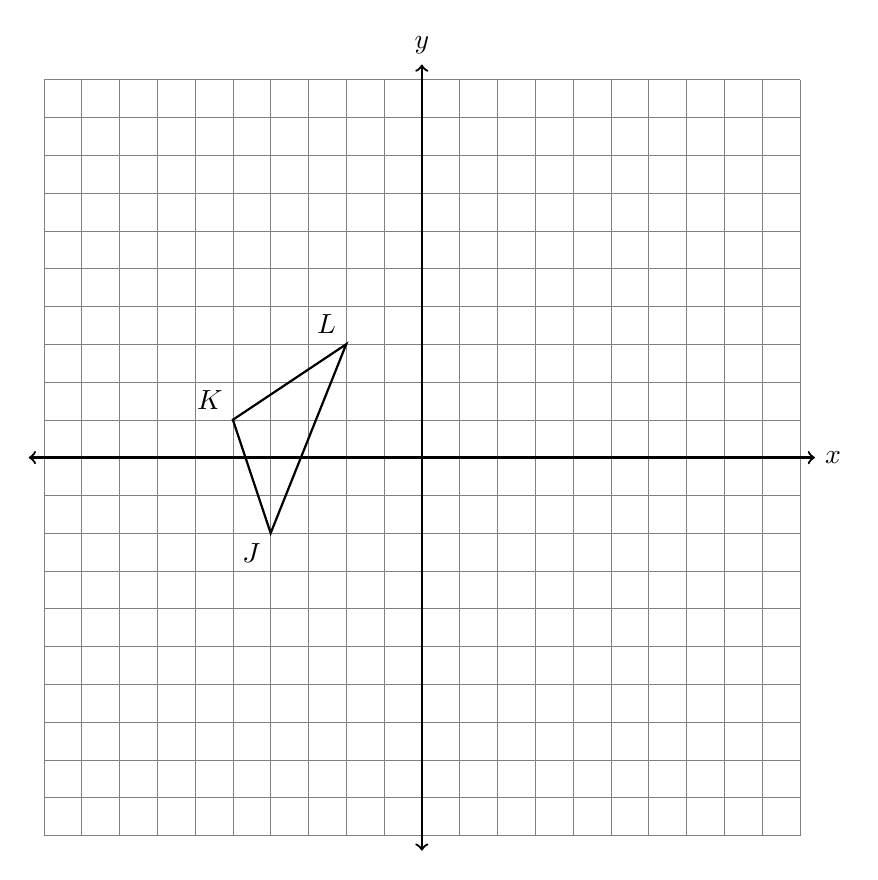
\begin{tikzpicture}[scale=.48]
       \draw [help lines] (-10,-10) grid (10,10);
       \draw [thick, <->] (-10.4,0) -- (10.4,0) node [right] {$x$};
       \draw [thick, <->] (0,-10.4)--(0,10.4) node [above] {$y$};

       \draw [thick]
       (-4,-2) node[below left] {$J$}--
       (-5,1) node[above left] {$K$}--
       (-2,3) node[above left] {$L$}--
       cycle;
     \end{tikzpicture}\\[1.5cm]

     \item Find the volume of a cone having a height of 12 feet and round base with a diameter of 3 feet. Express your result to the \emph{nearest cubic foot}. \vspace{5cm}

\newpage

     \item Find the area of parallelogram $ABCD$. The altitude $h$ of the parallelogram is 4.5 inches and the base $AB=7.15$ in.\\[1cm]
     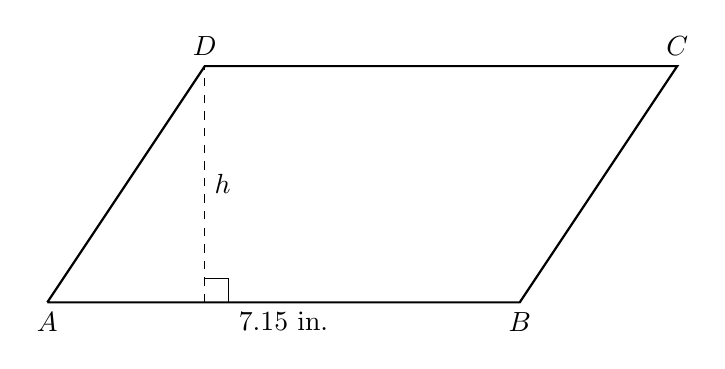
\begin{tikzpicture}%[scale=0.7]
       \draw [thick]
         (2,0)node[below]{$A$}--
         (8,0)node[below]{$B$}--
         (10,3)node[above]{$C$} --
         (4,3)node[above]{$D$} --(2,0);
      \draw [dashed] (4,0)--(4,3);
      \draw (4,0)++(0.3,0)--++(0,0.3)--+(-0.3,0);
      \node at (4,1.5)[right]{$h$};
      \node at (5,0)[below]{$7.15$ in.};
    \end{tikzpicture} \vspace{2cm}

    \item Find the volume of a sphere with a radius of 13 inches, to the \emph{nearest whole cubic inch}. \vspace{3cm}

    \item Circle $O$ has a radius of 5 inches, and two radii are drawn, $OA$ and $OB$, as shown. The radii are perpendicular, that is, $m\angle AOB=90^\circ$.\\
    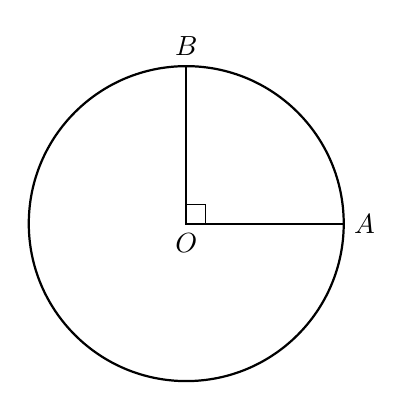
\begin{tikzpicture}[scale=0.4]
      \draw [thick] (0,0) node[below]{$O$} circle [radius=5];
      \draw [thick] (0,5) node[above]{$B$} --(0,0)--(5,0)node [right]{$A$};
      \draw (0,0)++(0.6,0)--++(0,0.6)--+(-0.6,0);
    \end{tikzpicture}
    \begin{enumerate}
      \item Find the circumference of circle $O$. \vspace{1.5cm}
      \item Find the length of the arc $\stackrel\frown{AB}$
      \end{enumerate}

\newpage

   \item Find the length of $\overline{AB}$, where $A(5,-6)$ and $B(13,0)$.
       \vspace{4cm}

   \item Determine relationship of each equation to the line  $y=\frac{4}{3} x-4$, circling either parallel, perpendicular, or neither.
     \begin{enumerate}
       \item $4x-3y=6$ \hspace{1cm} Parallel \qquad Perpendicular \qquad Neither
       \vspace{1.5cm}
       \item $3x+4y=5$ \hspace{1cm} Parallel \qquad Perpendicular \qquad Neither
       \vspace{2.cm}
     \end{enumerate}

  \item In the diagram below, $\overleftrightarrow{AC}$ has endpoints with coordinates $A(-1,2)$ and $C(9, -3)$.
    \begin{center} %4 quadrant regents grid
      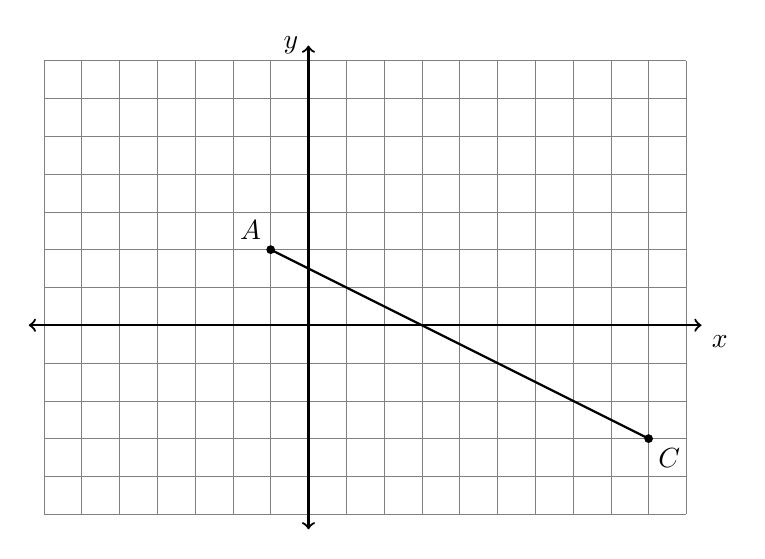
\begin{tikzpicture}[scale=.48]
        \draw [help lines] (-7,-5) grid (10,7);
        \draw [thick, <->] (-7.4,0) -- (10.4,0) node [below right] {$x$};
        \draw [thick, <->] (0,-5.4)--(0,7.4) node [left] {$y$};
        \draw [thick] (-1,2)--(9, -3);
        \draw [fill] (-1,2) circle [radius=0.1] node[above left] {$A$};
        \draw [fill] (9, -3) circle [radius=0.1] node[below right] {$C$};
      \end{tikzpicture}
    \end{center}
    If $B$ is a point on $\overline{AC}$ and $AB {:} BC = 2{:}3$,  what  are  the  coordinates of $B$?

\newpage

\item With a compass and straightedge, construct a hexagon inscribed in circle $O$. (Leave all construction marks.)
  \vspace{0.5cm}
  \begin{center}
  \begin{tikzpicture}
  \draw [thick] (0,0) circle [radius=4cm];
  \draw [fill] (0,0) circle [radius=0.05] node[below]{$O$};
  \end{tikzpicture}
  \end{center}

\vspace{1cm}

  \item Using  a  compass  and  straightedge,  construct  a perpendicular bisector of side $\overline{BC}$ in $\triangle ABC$ below.\\ (Leave all construction marks.)
    \vspace{0.5cm}
  \begin{center}
  \begin{tikzpicture}
    \draw [<->, thick]
      (0,0) node[left]{$A$}--
      (10,-2) node[right]{$B$}--
      (4,-5) node[below]{$C$}
      --cycle;
  \end{tikzpicture}
  \end{center}

\newpage
  \item Given  $\triangle EFG$ with $\overline{EF}$ extended to $A$. If $m\angle F=44^\circ$ and $m\angle G=92^\circ$, find $m\angle AEG$?
    \begin{center}
      \begin{tikzpicture}%[scale=0.7]
        \draw [thick](0,0)node[below]{$A$}--
          (2,0)node[below]{$E$}--
          (8,0)node[below]{$F$}--
          (4,3)node[above]{$G$} --(2,0);
      \end{tikzpicture}
    \end{center}

\vspace{4cm}

  \item In  $\triangle ABC$ shown below, $m\angle A=(5x+21)^\circ$, $m\angle B=(13x+4)^\circ$, and $m\angle C=(2x+15)^\circ$.\\[0.5cm] What is $m\angle A$?
  \begin{center}
      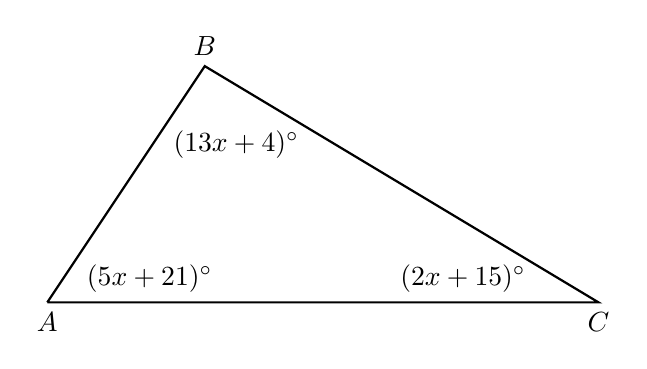
\begin{tikzpicture}
        \draw [thick]
          (2,0)node[below]{$A$}--
          (9,0)node[below]{$C$}--
          (4,3)node[above]{$B$} --(2,0);
          \node at (3.3,0)[above]{$(5x+21)^\circ$};
          \node at (8.2,0)[above left]{$(2x+15)^\circ$};
          \node at (4.4,2.3)[below]{$(13x+4)^\circ$};
      \end{tikzpicture}
    \end{center}

\end{enumerate}
\end{document}
